\documentclass[a4paper,10pt,ngerman]{scrartcl}
\usepackage{babel}
\usepackage[T1]{fontenc}
\usepackage[utf8x]{inputenc}
\usepackage[a4paper,margin=2.5cm,footskip=0.5cm]{geometry}
% Die nächsten vier Felder bitte anpassen:
\newcommand{\Aufgabe}{OOP-Projekt: Kartennavigation}
\newcommand{\Namen}{Jonathan Rajewicz}           % Namen der Bearbeiter/-innen dieser Aufgabe angeben
 
% Kopf- und Fußzeilen
\usepackage{scrlayer-scrpage, lastpage}
\setkomafont{pageheadfoot}{\large\textrm}
\lohead{\Aufgabe}
\cfoot*{\thepage{}/\pageref{LastPage}}

% Position des Titels
\usepackage{titling}
\setlength{\droptitle}{-1.0cm}

% Für mathematische Befehle und Symbole
\usepackage{amsmath}
\usepackage{amssymb}

% Für Bilder
\usepackage{graphicx}
\usepackage{wrapfig}

% Für Algorithmen
\usepackage{algpseudocode}

% Für Quelltext
\usepackage{listings}
\usepackage{color}
\definecolor{mygreen}{rgb}{0,0.6,0}
\definecolor{mygray}{rgb}{0.5,0.5,0.5}
\definecolor{mymauve}{rgb}{0.58,0,0.82}
\lstset{
  keywordstyle=\color{blue},commentstyle=\color{mygreen},
  stringstyle=\color{mymauve},rulecolor=\color{black},
  basicstyle=\footnotesize\ttfamily,numberstyle=\tiny\color{mygray},
  captionpos=b, % sets the caption-position to bottom
  keepspaces=true, % keeps spaces in text
  numbers=left, numbersep=5pt, showspaces=false,showstringspaces=true,
  showtabs=false, stepnumber=2, tabsize=2, title=\lstname,
  showstringspaces=false,
  literate={ö}{{\"o}}1 {ä}{{\"a}}1 {ü}{{\"u}}1 {ß}{{\ss}}1
}
\lstset{
extendedchars=\true,
inputencoding=utf8x
}
\lstdefinelanguage{JavaScript}{ % JavaScript ist als einzige Sprache noch nicht vordefiniert
  keywords={break, case, catch, continue, debugger, default, delete, do, else, finally, for, function, if, in, instanceof, new, return, switch, this, throw, try, typeof, var, void, while, with},
  morecomment=[l]{//},
  morecomment=[s]{/*}{*/},
  morestring=[b]',
  morestring=[b]",
  sensitive=true
}

% Diese beiden Pakete müssen zuletzt geladen werden
%\usepackage{hyperref} % Anklickbare Links im Dokument
\usepackage{cleveref}

\graphicspath{{./Bilder/}}

% Daten für die Titelseite
\title{\textbf{\Huge\Aufgabe}}
\author{\LARGE \Namen\\\\}
\date{\LARGE11. März 2024}
\begin{document}

\maketitle
\tableofcontents

\vspace{0.5cm}


\section{Problemstellung und Kundenanforderungen}
Bei der Aufgabe handelt es sich um ein 3-dimensionales bin packing problem, bei dem eine gegebene Menge von Quadern in einen Würfel platziert werden, wobei ein Würfel schon platziert ist. Im folgenden wird die Kiste in “Plätze” aufgeteilt, wobei ein Platz die Maße (1,1,1) hat. Damit ist das Problem NP-schwer, weshalb ein Brute-Force-Verfahren genutzt wird. Zur Lösung wird zunächst ein Quader in Ebene 0 in der Ecke hinten links platziert. Dabei gibt es 3!=6 Möglichkeiten von Drehungen (es müssen keine Drehungen, bei dem der Quader nach unten, nach links oder nach hinten ausgedehnt,  beachtet werden, da beim genannten Startpunkt begonnen wird). Nun wird der nächste freie Platz, bei dem alle unteren, linken und hinteren Plätze bereits belegt sind, von einem noch nicht benutzten Quader belegt. Dies wird so oft durchgeführt, bis alle Quader verwendet wurden, also eine Lösung gefunden wurde. Dies funktioniert nach dem Prinzip der Tiefensuche, da wenn keine Lösung für eine Anordnung gefunden wurde, zunächst der als letztes platzierte Würfel durch andere noch verfügbare ersetzt wird, wenn hier keine Lösung gefunden wurde, dann der vorletzte usw. Der Platz des goldenen Würfels ist von Anfang an belegt. Im Worst-Case ergibt sich damit eine Laufzeit von $\mathcal{O}(n!)$, wenn alle möglichen Anordnungen von Quadern betrachtet werden müssen.

\newpage
\section{Planung}
\begin{figure}[!ht]
  \center
  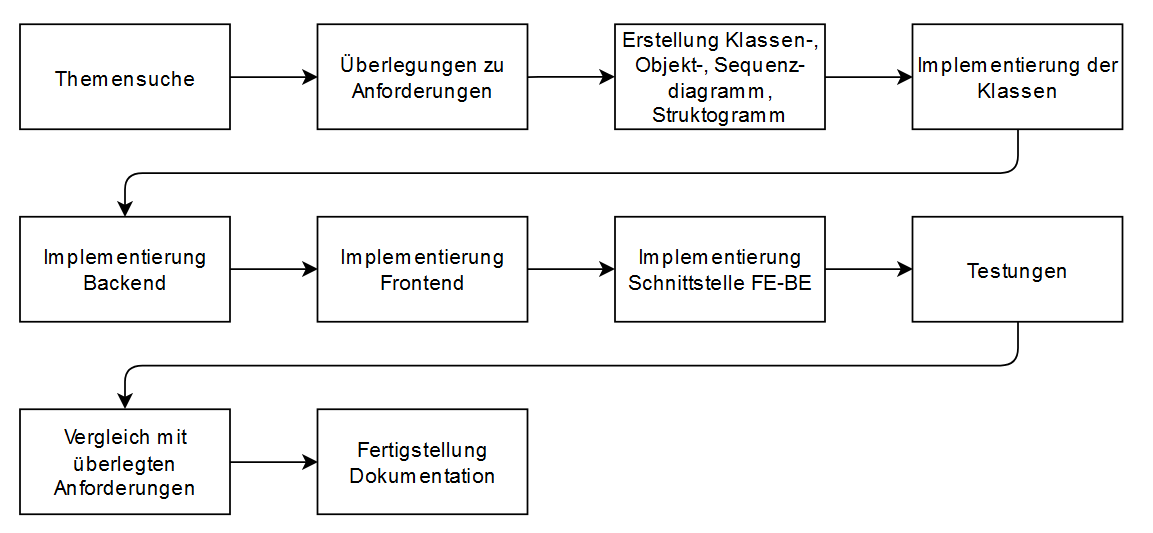
\includegraphics[width=\textwidth]{Pipelinediagramm.png}
  \vspace{-.5cm}
  \caption{Pipelinediagramm}
\end{figure}

\section{Analyse informatischer Anforderungen}
ere

\newpage
\section{Diagramme}
\begin{figure}[!ht]
  \center
  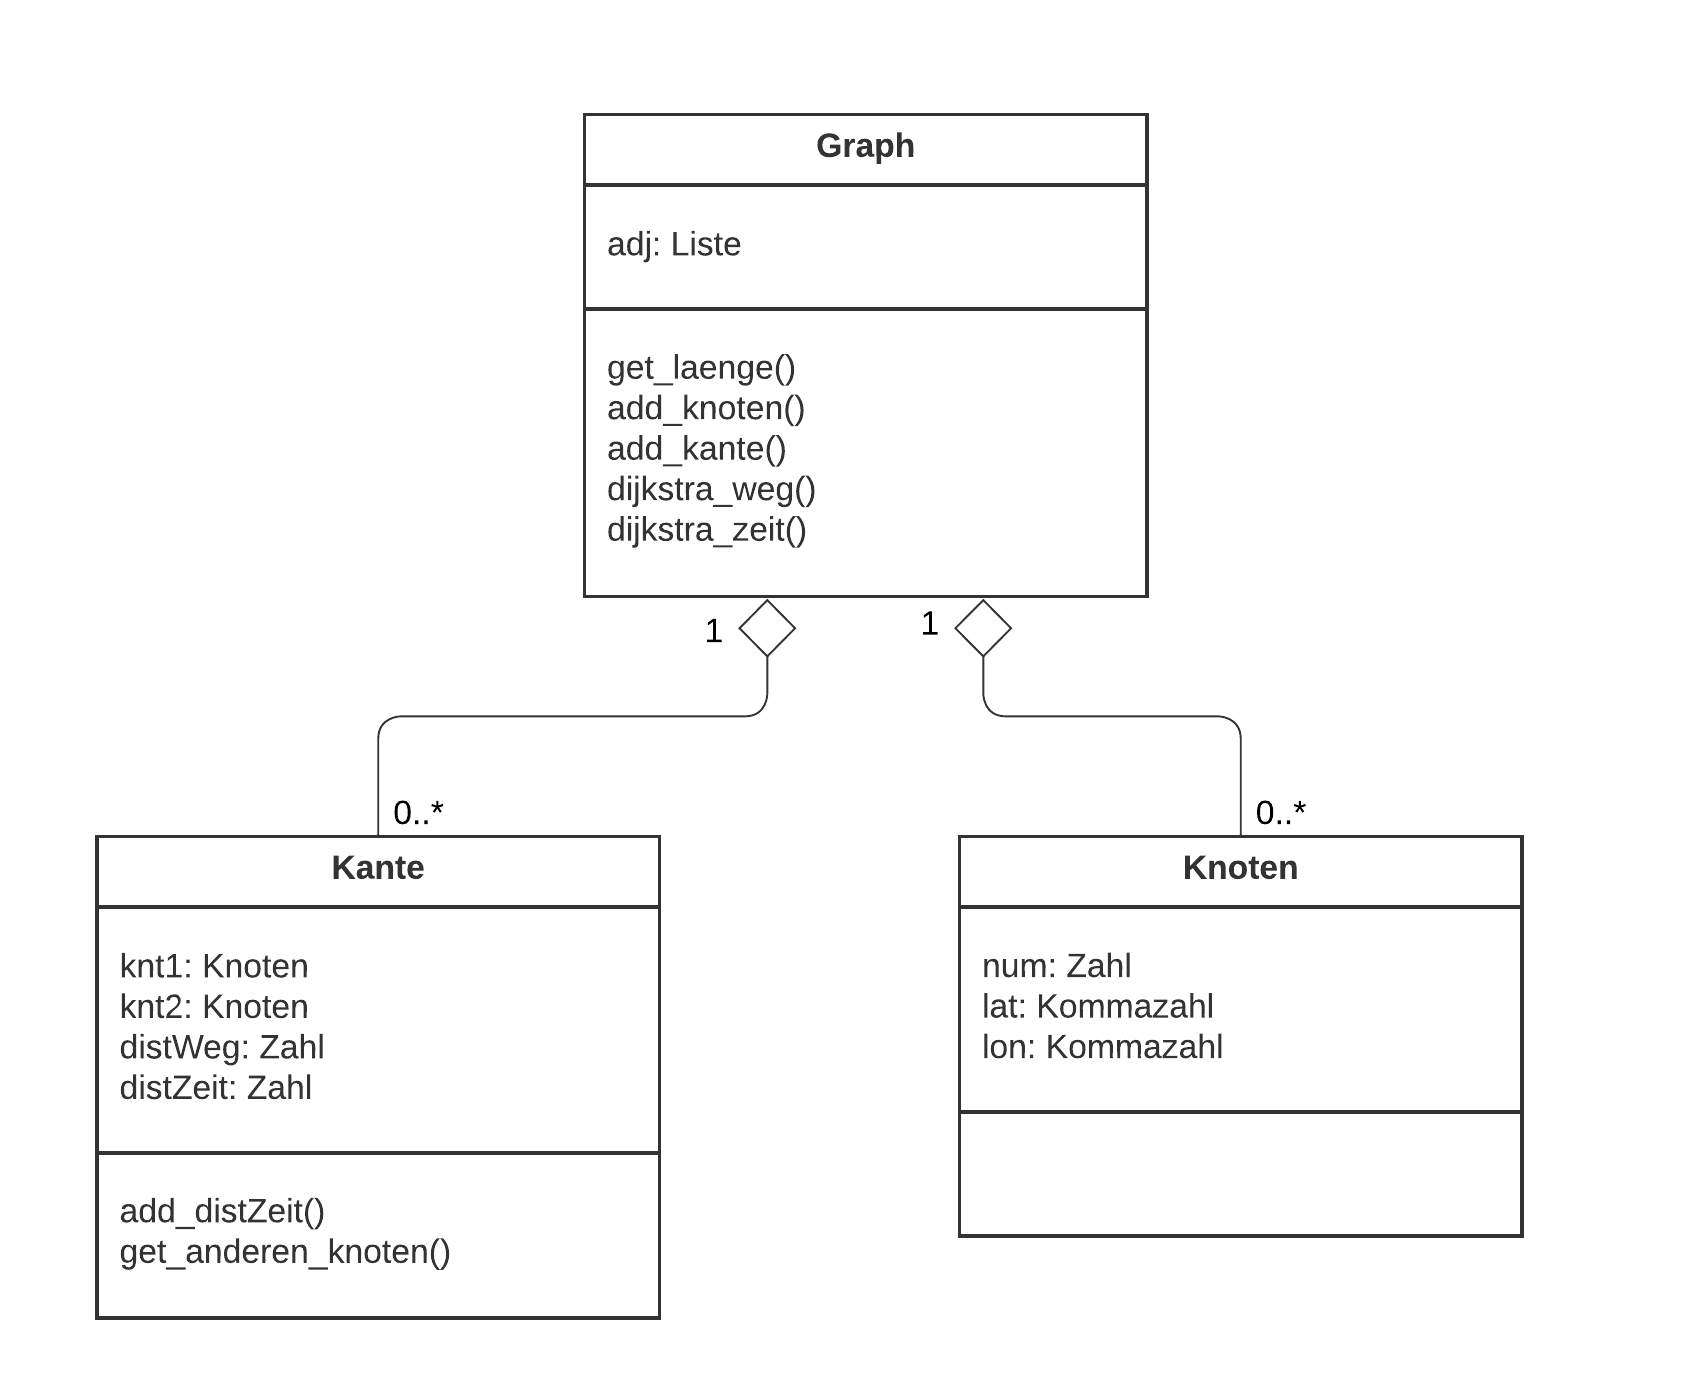
\includegraphics[width=\textwidth]{Klassendiagramm.png}
  \vspace{-.5cm}
  \caption{Klassendiagramm}
\end{figure}

\begin{figure}[!ht]
  \center
  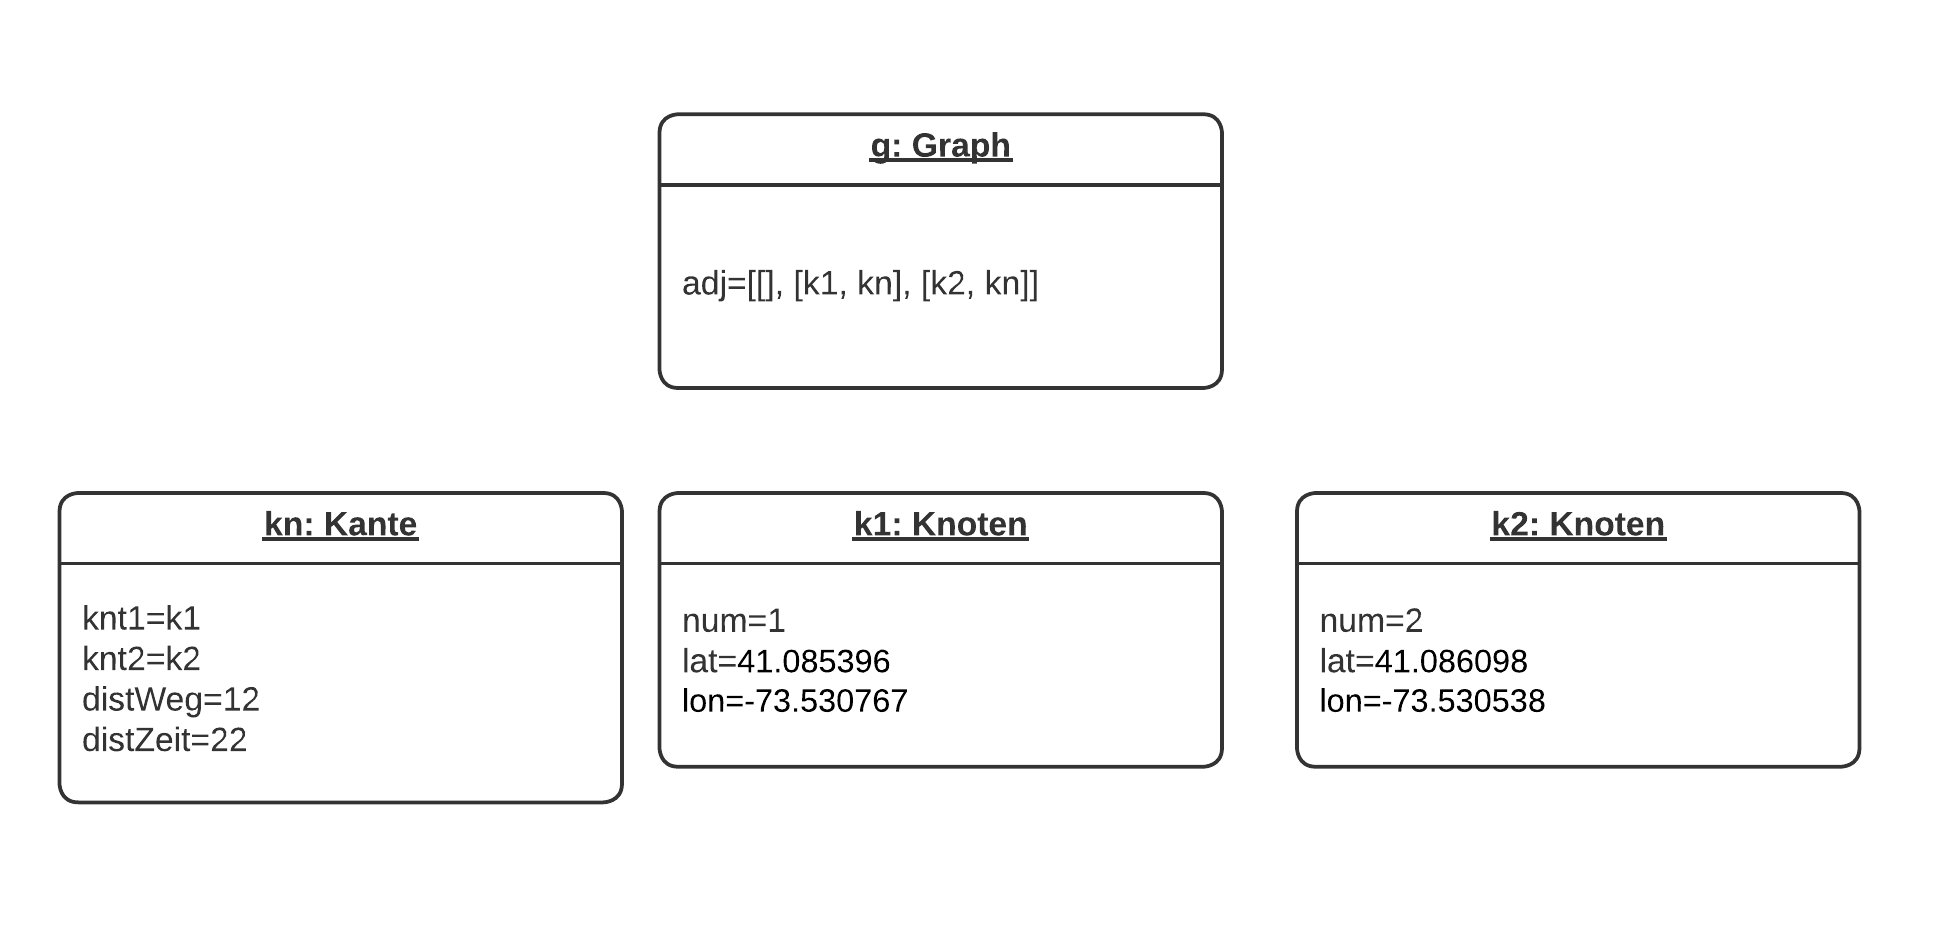
\includegraphics[width=\textwidth]{Objektdiagramm.png}
  \vspace{-1cm}
  \caption{Objektdiagramm}
\end{figure}

\begin{figure}[!ht]
  \center
  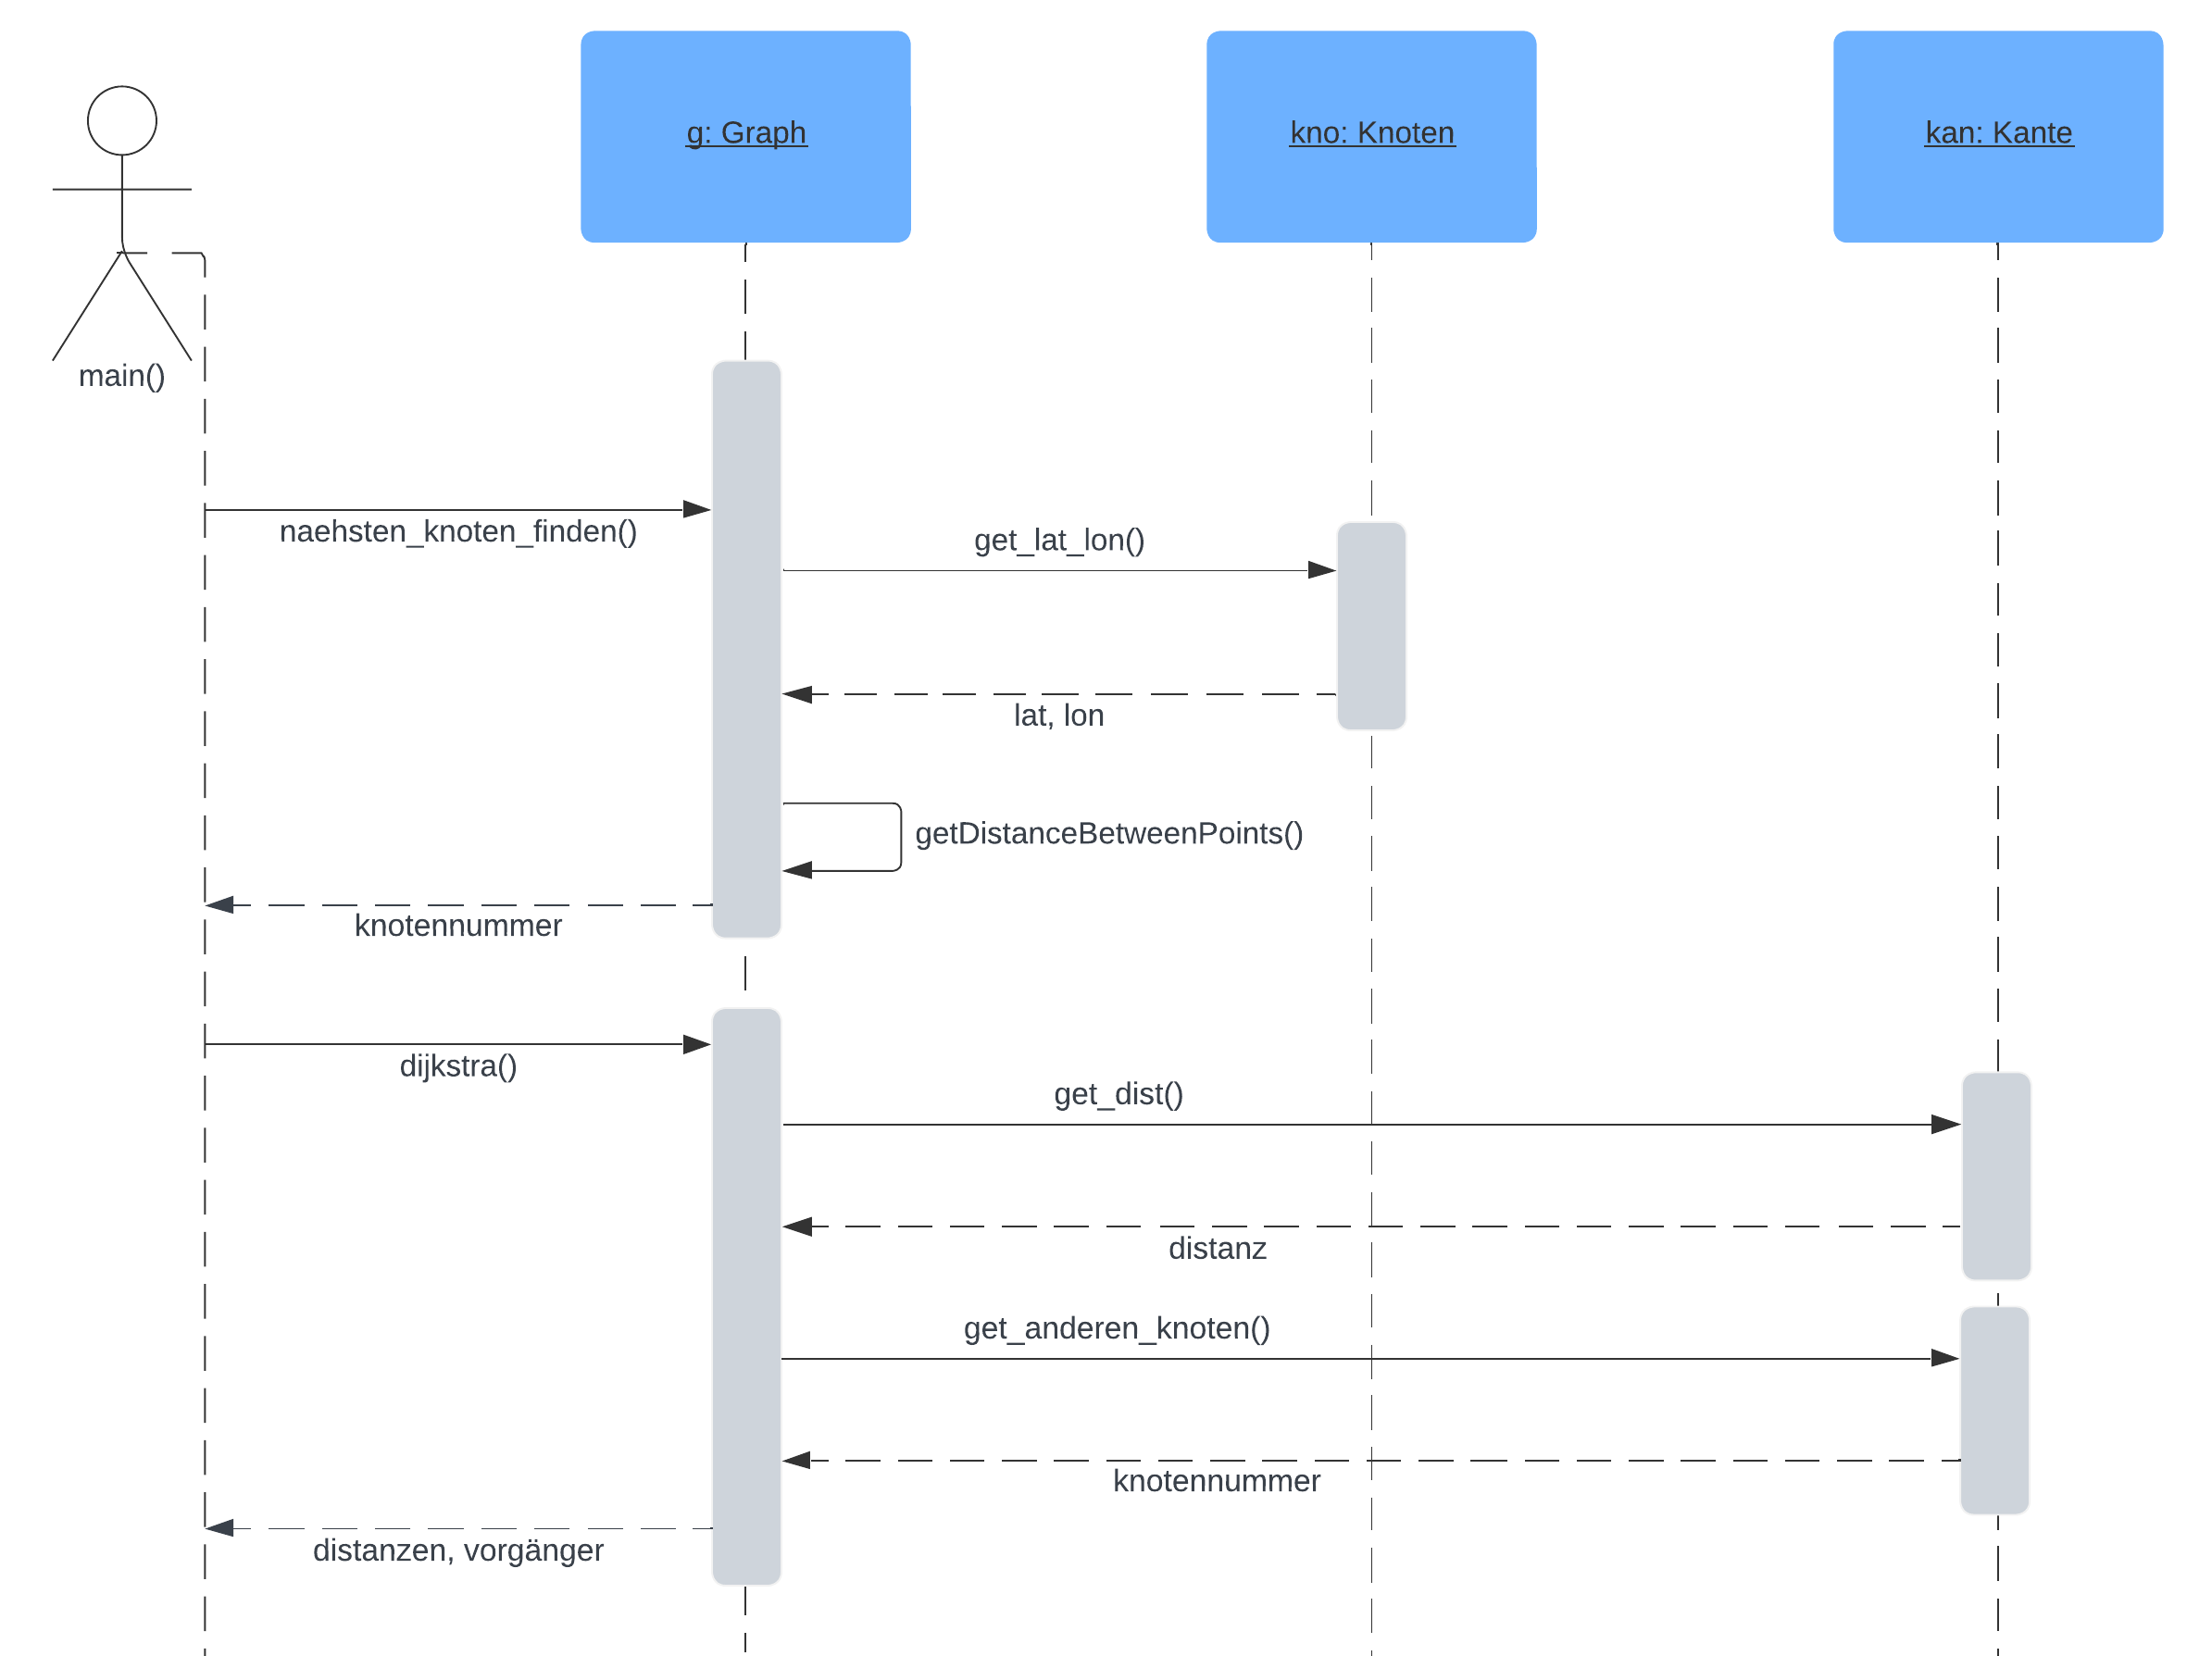
\includegraphics[width=\textwidth]{Sequenzdiagramm.png}
  \vspace{-.5cm}
  \caption{Sequenzdiagramm}
\end{figure}

\begin{figure}[!ht]
  \center
  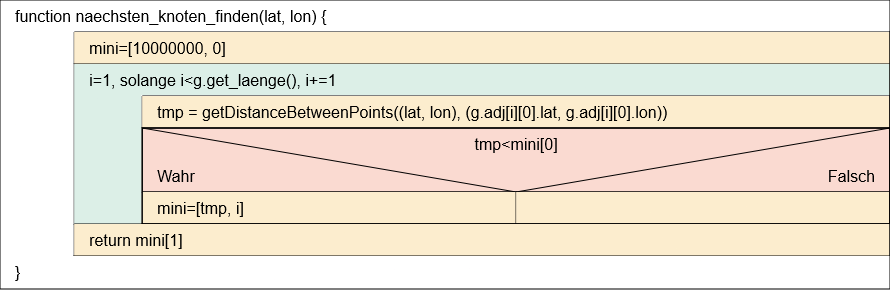
\includegraphics[width=\textwidth]{Struktogramm.png}
  \vspace{-1cm}
  \caption{Struktogramm für $naechsten\_knoten\_finden()$}
\end{figure}

\newpage
\section{Umsetzung}
d fghgh fghfgh fg

\end{document}
